\documentclass[draft]{beamer}

\usepackage[orientation=landscape, size=a0, scale=1.4, debug]{beamerposter}
\usepackage{booktabs}
\usepackage{dcolumn}
\usepackage{colortbl}
\usepackage{xcolor}
\usepackage{hyperref}
\usepackage{amsmath}
\usepackage[absolute, showboxes, overlay]{textpos}
%\usepackage[absolute, overlay]{textpos}
\usepackage{calc}
\usepackage[colorgrid,texcoord]{eso-pic}
\usepackage[bibstyle=numeric,maxcitenames=6]{biblatex}

% \defaultfontfeatures{Mapping=tex-text}
\usepackage{pifont}
\usepackage{algorithm}
\usepackage[noend]{algpseudocode} 
\usepackage{mathtools}
\usepackage{array}
\usepackage{color}
\usepackage[export]{adjustbox}
\usepackage{multirow}
\usepackage{dsfont}
\usepackage{bm}
\usepackage{xcolor}

% \newcolumntype{L}[1]{>{\raggedright\let\newline\\\arraybackslash\hspace{0pt}}m{#1}}
% \newcolumntype{C}[1]{>{\centering\let\newline\\\arraybackslash\hspace{0pt}}m{#1}}
% \newcolumntype{R}[1]{>{\raggedleft\let\newline\\\arraybackslash\hspace{0pt}}m{#1}}

\usetheme{enziteto}

\addbibresource{../referomnia/referomnia.bib}

\usepackage{blindtext}

% \newcommand*\mccol[2]{\multicolumn{#1}{c}{#2}}
% \newcommand*\tmccol[2]{\mccol{#1}{\tiny\textsf{#2}}}
% \newcommand*\bmccol[2]{\mccol{#1}{\textbf{#2}}}
\newcommand{\argmax}{\operatornamewithlimits{argmax}}
\newcommand{\argmin}{\operatornamewithlimits{argmin}}
\newcommand{\nodeset}[1]{\bm{\mathsf{#1}}}

\definecolor{lacamgreen} {RGB} {72, 175, 115}
\definecolor{lacamlilac} {RGB} {107,93,153}
\definecolor{lacamlilac2} {RGB} {93, 109, 152}
\definecolor{lacamlightlilac} {RGB} {174, 166, 201}
\definecolor{lacamdarklilac} {RGB} {51, 10, 102}
\definecolor{lacamgold} {RGB} {255, 87, 0}
\definecolor{lacamdarklilac5} {RGB} {51, 10, 102}
\definecolor{lacamgold5} {RGB} {255, 87, 0}
\definecolor{violet} {RGB} {119, 111, 178}
\definecolor{petroil2} {RGB} {36, 165, 175}
\definecolor{petroil4} {RGB} {30, 132, 149}
\definecolor{petroil6} {RGB} {23, 101, 115}
\definecolor{gold2} {RGB} {255, 130, 0}
\definecolor{gold4} {RGB} {250, 100, 0}
\definecolor{gold6} {RGB} {245, 90, 0}

\newcommand{\highlight}[2][yellow]{\mathchoice%
  {\colorbox{#1}{\strut\textcolor{white}{$\displaystyle{#2}$}}}%
  {\colorbox{#1}{\strut\textcolor{white}{$\textstyle{#2}$}}}%
  {\colorbox{#1}{\strut\textcolor{white}{$\scriptstyle{#2}$}}}%
  {\colorbox{#1}{\strut\textcolor{white}{$\scriptscriptstyle{#2}$}}}}%

\def\restrict#1{\mkern 1mu \vrule height 1.3ex\mkern2mu #1}

\makeatletter
\def\maketag@@@#1{\hbox{\m@th\normalfont\small#1}\hspace{30pt}}
\makeatother

% 
% custom colors
\definecolor{untractable_red}{RGB}{209, 25, 25}
\definecolor{tractable_green}{RGB}{0, 153, 51}

\newcommand{\cmark}{\ding{51}}%
\newcommand{\xmark}{\ding{55}}

\newcommand{\summark}{\tiny\textcolor{lacamlilac}{$\boldsymbol{\oplus}$}}
\newcommand{\prodmark}{\tiny\textcolor{lacamlilac}{$\boldsymbol{\otimes}$}}

\setbeamertemplate{itemize item}{\raisebox{.21ex}{\hbox{\summark}\hspace{0pt}}}
\setbeamertemplate{itemize subitem}{\raise .2ex\hbox{\prodmark}\hspace{0pt}}
\setbeamertemplate{itemize subsubitem}{\textcolor{lacamlilac}{$\oplus$}}
% \setbeamertemplate{bibliography item}{\hspace{10pt}\raise
%   .2ex\hbox{\tiny\textcolor{lacamlilac}{$\boldsymbol{\oplus}$}}\insertbiblabel}
\setbeamertemplate{bibliography item}{\insertbiblabel}


\setbeamertemplate{headline}{}

% \addbibresource{../referomnia/referomnia.bib}

\title{Fast and Accurate Denstiy Estimation with Extremely Randomized
  Cutset Networks}
\author{Nicola  {Di Mauro}, Antonio  Vergari, Teresa M.A. Basile and Floriana Esposito}
\date{}


\begin{document}

\institute{Università degli Studi di Bari}
% \department{Dipartimento di Informatica}
% \laboratory{LACAM}
% \group{Machine Learning}

% \institutelogo{
\includegraphics[width=25pt]{figures/unibaba}}
% \lablogo{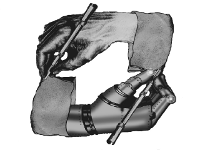
\includegraphics[width=35pt]{figures/lacam}}


% {
%   \setbeamertemplate{headline}{}
%   \setbeamertemplate{footline}{}
%   \begin{textblock}
%     \titlepage
%   \end{textblock}
% }

\newcommand{\hmargin}{30mm}
\newcommand{\vmargin}{30mm}
\textblockorigin{\hmargin}{\vmargin}

\setlength{\TPHorizModule}{1cm}
\setlength{\TPVertModule}{1cm}

%
% TODO: generalize this
\newlength{\posterwidth}
\newlength{\posterheight}
\setlength{\posterwidth}{1189mm}
\setlength{\posterheight}{841mm - 2\hmargin}

\newcommand{\ncols}{3}
\newlength{\colwidth}
\setlength{\colwidth}{\posterwidth/\ncols}

\newlength{\colhpoint}
\setlength{\leftmargini}{35pt}


\begin{frame}{}
  %
  % title
  % \textblockcolour{header}
  \begin{textblock}{78}(0, 0)
    \usebeamerfont{section name}
    \Huge
    Fast and Accurate Density Estimation with\\
    Extremely Randomized Cutset Networks
  \end{textblock}
  %
  % authors
  \begin{textblock}{40}(70, 0.5)
    \usebeamerfont{author}
    \small
    Nicola {Di Mauro}${}^{\text{\summark}}$\\[5pt]
    Antonio Vergari${}^{\text{\summark}}$\\[5pt]
    Teresa M. A. Basile${}^{\text{\prodmark}}$\\[5pt]
    Floriana Esposito${}^{\text{\summark}}$
  \end{textblock}
  % 
  % email
  \begin{textblock}{30}(81, 0.6)
    %\usebeamerfont{author}
    \small
    \emph{nicola.dimauro@uniba.it}\\[5pt]
    \emph{antonio.vergari@uniba.it}\\[5pt]
    \emph{teresamaria.basile@uniba.it}\\[5pt]
    \emph{floriana.esposito@uniba.it}
  \end{textblock}
  %
  % affiliations
  \begin{textblock}{30}(90.5, 0)
    \usebeamerfont{author}
    \scriptsize
    \begin{minipage}[t]{5cm}
      \vspace{0pt}\hspace{15pt}
      
\includegraphics[width=110pt]{figures/unibaba}
    \end{minipage}\hspace{-5pt}
    \begin{minipage}[t]{15cm}
    \vspace{30pt}
      \flushleft
      % University of Bari, Italy\\
      University of Bari\\
    \vspace{2pt}
    % Computer Science Department
    LACAM - Machine Learning
    \end{minipage}\\[0.75cm]
    \usebeamerfont{author}
    \scriptsize
    \begin{minipage}[t]{5cm}
      \vspace{-5pt}
      % 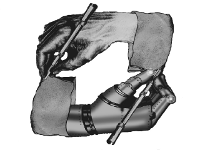
\includegraphics[width=145pt]{figures/lacam}
      %\hspace{28pt}\includegraphics[width=95pt]{figures/cam-logo-big-gray.png}
    \end{minipage}\hspace{-5pt}
    \begin{minipage}[t]{15cm}
      \vspace{20pt}
      \flushleft
      % LACAM Laboratory\\
      University of Cambridge\\
      \vspace{2pt}
      % Machine Learning
      Department of Engineering
    \end{minipage}
  \end{textblock}
  
  
  %
  % section 1
  \begin{textblock}{30}(0, 9.5)
    \usebeamerfont{section name}
    Density estimation \dots
  \end{textblock}

  %
  % section 1
  \begin{textblock}{30}(35, 9.5)
    \usebeamerfont{section name}
    Cutset Networks \dots
  \end{textblock}

  
    \begin{textblock}{180}(10, 105.)
    \usebeamerfont{section name}
    Bomba
  \end{textblock}
  
  % 
  % section 5
  \begin{textblock}{80}(0, 105.)
    \usebeamerfont{section name}
    References
  \end{textblock}

  
 \begin{textblock}{52}(0, 107.5)
    \small
    % \blindtext
    \setlength\bibitemsep{8pt}
    \printbibliography[heading=none]
  \end{textblock}
  
  \begin{textblock}{25.2}(27.4, 107.5)
    \small
    % \blindtext
  \end{textblock}
  
  % \begin{textblock}{25.2}(54.2, 105.8)
  %   \small
  %   % \blindtext
  % \end{textblock}

  % 
  % footer
  \begin{textblock}{80}(0, 77.3)
    \usebeamerfont{subtitle}
    \small
    \textbf{ECML-PKDD 2017}  -  18th-22rd September 2017, Skopje, Macedonia\hfill
    {\url{https://github.com/nicoladimauro/cnet}}\ \ $\cdotp$ \ \
    {\url{https://github.com/nicoladimauro/dcsn}}
  \end{textblock}
  
\end{frame}


\end{document}

%%% Local Variables:
%%% mode: xetex
%%% TeX-master: t
%%% End:
